\documentclass{article}
\usepackage{amssymb,amsthm,amsopn,amsmath,amscd,graphicx}
\usepackage[authoryear,round]{natbib}
\usepackage[mathscr]{euscript}
\usepackage{url}
\usepackage{float}
\usepackage{booktabs}
\setlength{\textwidth}{6.5in}
\setlength{\textheight}{9.0in}
\hoffset=-0.80in
\voffset=-1.00in

\begin{document}

\title{Conversation as skilled behavior: How conversational trajectories change with expertise}
\author{Yume Ishida \& Jeff Yoshimi}
\date{\today}
\maketitle

\begin{abstract}
TODO

\textbf{Keywords:} expertise; conversation; semantic space; skilled behavior
\end{abstract}

\section{Introduction}

Skilled behavior involves a process of contraction and ramification in a behavioral space. On the one hand, particular actions become increasingly refined as a person gains expertise. This is often described as a reduction in behavioral variability or degrees of freedom (what is described by standard learning curves), and can be visualized in terms of measured bodily states occupying less of a behavioral space over time \citep{vereijken1992freezing,adolph2015intraindividual}. For example, after learning to perform a basic kick, trajectories in the space of joint positions for a kick will occupy much less of that space. On the other hand, as a person develops expertise, they develop an ability to respond flexibly to situations. They can kick a ball in more ways and in response to unusual situations. Thus, variability is reduced action by action, but it is also ramified and in some cases increased \citep{wilson2008coordination,adolph2015intraindividual}. Some studies have found U-shaped curves when comparing performance at different levels \citep{wilson2008coordination,busquets2016differing}, which suggest an initial reduction in variability followed by fine-tuning which increases variability: `In the final stages of developing a skilled performance, a functional variability is accessed that brings flexibility to the system allowing it to cope with perturbations'' \cite{wilson2008coordination}. As a recent review puts the point like this: ``Skilled performance is characterized by a dual capacity: reducing variability in performance-critical parameters to ensure consistency, while simultaneously leveraging functional variability to adapt to dynamic demands.'' \citep{tsunoda2026relationship}

It is natural to suppose that the changes in behavioral space associated with skill acquisition should be mirrored in semantic spaces as people learn to speak about specific topics. They learn the correct ways to say specific things---technical terms and common phrases---but also learn how to talk about more things in more ways. Compare someone talking about Russian history who has just learned the basics with someone who has studied and taught the topic for 30 years: the latter will speak more naturally and fluently and will be able to field a wide variety of questions with ease. This suggests a parallel to behavioral skill spaces: expert conversation should occupy less of a semantic space but also be more ramified.

% Much of this was not framed as "cognitive skills", but simply learning, problem solving, etc. Much of it also came _before_ physical skill
There is a literature on cognitive skills that has established many parallels between domains of cognition and physical skill: fluency and speed increase, while error rates decrease, in mathematics, problem solving, reading, and related activities as people learn to perform them \citep{groot_thought_1965,robinson_mathematical_1978,egan_chunking_1979,chi1981expertise}. There has, however, been relatively little analysis of conversation from this perspective. This is regrettable, especially given the widespread availability of tools and techniques for studying semantic spaces.

In this exploratory study, we examine this question using a publicly available WIRED dataset in which experts explain scientific topics to listeners at five levels of expertise. The conversations concern a variety of scientific topics, and each expert-listener exchange lasts only a few minutes. Using a large sentence-embedding model and standard latent-semantic-analysis (LSA)-style techniques, we explore the comparative structure of conversational spaces across these dyads. We find support for the idea that variability is both reduced and ramified in experts' semantic spaces.

% Once this framing is settled, material on semantic alignment can be worked back into the paper, especially where it helps distinguish contraction from successful expert--listener coordination.
% We should have a look at the literature on fluency and billingualism as well.

\section{Methods}

This is an exploratory analysis. We considered a number of candidate measures and feature-selection strategies before focusing on the measures reported below. 
% Describe in particular our earlier null results with network/graph techniques

\subsection{Data and Procedure}

A set of 14 videos were selected from the “5 levels” playlist published by WIRED, a series that has an expert explain a concept in their *** field of expertise at 5 levels: to a child, a teenager, an undergraduate college student, a graduate student, and a fellow expert. 

% Probably no need to report the abandoned method
% Yume: citation for Sentence Transformers.  Also, a few paragraphs down mentions another embedding. Which was it? ALSO, the last paragraph in this section is also a bit redundant.
The auto-generated transcripts on the Youtube platform were processed by Gemini*** along with the video data to assign speaker labels to each utterance, or to chatGPT to assign speaker labels contextually (this method ended produced mixed results, and was therefore abandoned after a few videos). All speaker pair corpora were reformatted into CSV format with columns for sequence, speaker, utterance, and notes. The CSV files for each video were broken up into five separate files, one for each speaker pair. Within each speaker-pair CSV, utterances were assigned embeddings using SentenceTransformers, which were used to calculate a variety of statistics for each conversation/speaker pair. SentenceTransformers we deemed an effective embedding model, as sentence embeddings would most accurately capture the conceptual/semantic characteristics of each utterance, and therefore be *** representative of each single semantic act. Sentences (and utterances in our case) represent the smallest linguistically stable unit of propositional meaning, allowing each embedding to correspond to a single semantic contribution while preserving sufficient contextual richness for distributional analysis. We also analyzed trigram embeddings (since utterance lengths are relatively uneven), which were put through the same pipeline as the sentence embeddings. *
% Prob no nee d to mention alternate embeddings unless there is a clear story about how they had a problem that the current method overcame.

% Yume you made various pictures of these encoding styles. I wouldn't mind bringing a few of them back. Where can I find them? Maybe this can be my next task. Or tell me how to generate them from the code. ideally at the command line without having to open a notebook
Let the two speakers in a conversation be denoted by $A$ and $B$ and conversational turn by $t$.  Utterances were defined as short, semantically coherent segments derived from the transcript, rather than strictly as full speaker turns or grammatical sentences. In practice, segmentation was performed manually by identifying units that expressed a single idea or communicative function. Boundaries were introduced at natural breakpoints such as pauses, interruptions, or shifts in semantic content, such that a single speaker turn $t$ could contain multiple utterances.

This approach was adopted to better align the unit of analysis with the embedding-based metrics used in this study. Because sentence embeddings operate over semantically meaningful units, segmenting transcripts into smaller, coherent utterances allows for more fine-grained representation of local conversational dynamics than would be possible using full turns alone. We embedded the utterances in turn $t$ in a 384-dimensional real vector space using the model \texttt{all-MiniLM-L6-v2} and denote this embedding $e_t^A$ for speaker $A$ and $e_t^B$ for speaker $B$. This makes it possible to show conversations as unfolding sequences of points in a space, as illustrated in figure \ref{fig:embedding}. Speaker identity is coded by color.

We encode expertise using ordinal variables $E_A, E_B \in \{0,1,2,3,4\}$, corresponding to child, teen, college student, graduate student, and expert, respectively. We define the absolute expertise gap between $A$ and $B$ as
\begin{equation}
|\Delta E| = |E_B - E_A| .
\end{equation}
and signed expertise gap as
\begin{equation}
\Delta E = E_B - E_A ,
\end{equation}
The absolute gap ranges from 0 to 4 where 0 corresponds to matched expertise and 4 is the maximum possible expertise gap. The signed gap ranges from -4 to 4 with negative values indicating $A$ has more expertise and positive values indicating $B$ has more expertise.

The WIRED transcripts were put in CSV format with columns for sequence, speaker, text, and notes, and each row dedicated to a single utterance. Utterances were defined as relatively short, semantically coherent segments that expressed a single idea or communicative function, derived from each speaker turn, rather than as full turns or full grammatical sentences. Turns were segmented at natural break points such as pauses, interruptions, or stark shifts in semantic content. The utterances were embedded using the model all-MiniLM-L6-v2, which returns 384-dimensional vectors per input (per utterance in our case). For every time step (every utterance), the embedding assigned to the utterance was notated as et.

\subsection{Metrics}

% For each of these, Jeff can add simple plain-english up front. Some pictures would also be nice. Once we have settled on the technique for generating them we can decide which ones to add.

To capture the general distribution of embeddings across conversations, we looked at centroid distances and a number of dispersion metrics. To calculate centroid distances, we first calculated the centroids at the final state of the conversation sequence (formulas for centroids) and calculated Euclidean distances between the centroid pairs (formula for distance). The metric captures the general distance between the totality(?) of the embedding points of the two interlocutors, reflective of the difference of the “average” semantic use between speakers. Smaller distances would be indicative of generally similar semantic use versus larger distances which would indicate dissimilar semantic use.

Radial distances (q10, median, q90) from the conversation centroids were also calculated to examine the dispersion of embeddings relative to the conversation’s “average” embedding (with an emphasis on q90 distances). The centroid of each conversation was calculated as (formula), and distances were calculated as (formula). Lower q10 distances would be indicative of conceptual tightness, ***** and potential repetition. Lower q90 distances would indicate greater semantic cohesion and (maybe) contraction, as even the furthest embeddings in the distribution would be relatively close to the conversation’s conceptual center.

Dimensional analysis was performed to capture the organization of variance across different directions. Participation ratio (formula) is essentially a “count” of how many eigenvalues(principal components) share the embeddings’ variance. The embeddings are centered around the conversation centroid and are put into a covariance matrix. In essence, we are simply examining the dimensional structure of the embeddings, disregarding location. (The covariance matrix is decomposed using SVD, with each eigenvector representing a principal component, and its corresponding eigenvalue represents the amount of variation is ****. The eigenvalues are then normalized, so that each normalized eigenvalue represents the percentage of the total semantic variation that is accounted for by that direction. Participation ratio is the ratio of square of total variance over the sum of squared variances along the individual directions).  A participation ratio of 1 would indicate the variance lies in one direction. Higher participation ratios would indicate the variance being shared by more dominating directions. In interpretation, this could be indicative of organized movement across a greater number of semantic directions.

\section{Results}

The analyses provide preliminary confirmation of the contraction-and-ramification hypothesis.

\subsection{Centroid Distances}
Figure~\ref{fig:centroid-distances} shows the distances between speaker centroids by partner expertise level. Centroid distances decreased as expertise gap decreased by$\beta = -0.313$ per expertise level, 95\% CI $[-0.414, -0.211]$(adjusted, from the fitted REML model) with expert-expert conversations having the smallest centroid distances. Running a parametric bootsrak likelihood-ratio test, we found that the differences by expertise were statistically significant and unlikely under the null LR = 11.4, \textit{p} = .001. Even after applying Benjamini-Hochberg correction, the *** survived $p_{\mathrm{FDR}} = .002$.This indicates that as partner expertise increases, the overall semantic usage of the two interlocutors becomes significantly more similar. This would make sense, as expert-expert pairs(for example) are operating very much “in the same space,”  with access to the same concepts and by extension, vocabulary, as opposed to expert-novice pairs where unlike their expert partners, novice speakers have limited vocabulary and access to concepts. Expert-novice conversations also tend to require extensive scaffolding, as novices often have very limited knowledge of the concepts being discussed. The concepts of discussion have to be explained with simpler, more digestible language without overloading the conversation with technical jargon. The expert is required to scaffold, with the aim of getting the novice “on the same page/in the same kind of space(information organization).” The novice utterances tend to simply answer expert questions, and will use words outside of the topic's technical vocabulary, whereas experts may use some technical words when introducing ideas making the average embedding(centroid) of the speakers further. Experts do not have to undergo this scaffolding process (more semantic precision).

\begin{figure}[H]
    \centering
    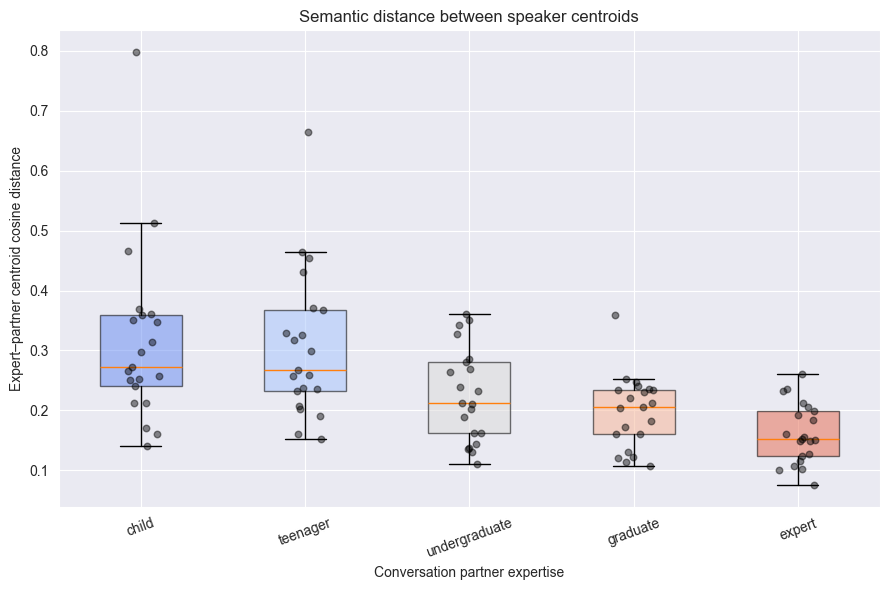
\includegraphics[width=0.85\linewidth]{figures/centroid_distances_plot.png}
    \caption{Cosine distance between expert and partner semantic centroids by conversation partner expertise.}
    \label{fig:centroid-distances}
\end{figure}

\subsection{Radial Distances}

Figures~\ref{fig:radial-distance-median} and~\ref{fig:radial-distance-q90} show the median and 90th-percentile radial distances, respectively. Embedding distributions tended to shift with expertise, with median radial distances decreasing by $\beta= -0.133$ per level increase, 95\%CI$[-0.239,-0.027]$, and q90 distances increasing by $\beta= 0.106$ per level increase, 95\%CI$[-0.003,-0.214]$, though not statistically significant,$p_{\mathrm{FDR}}= .025$ and $p_{\mathrm{FDR}} = .083$, respectively . Expert distributions tended to have slightly more concentration near the centroid (which could indicate high specificity, but could be confounded with redundancy), but also explored enough relative to the conversational center(or it could be something else) to have further points in the periphery. Novices, on the other hand, had slightly less concentration near the centroid and closer peripheral embeddings.
% probably put this somewhere later: We can see through these changes in distribution how conversations tend to "pull together" (with closer centroids and smaller median radial distances) and expand or "reach out" (with larger PR and greater q90 radial distances) as partner expertise increased

\begin{figure}[H]
    \centering
    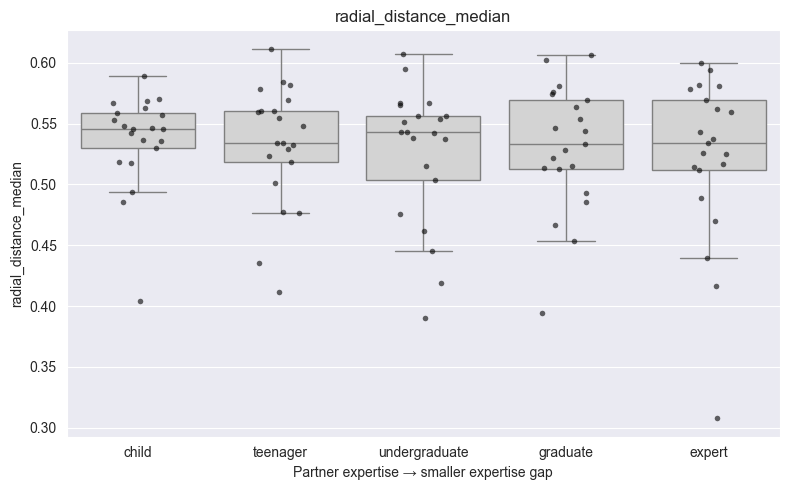
\includegraphics[width=0.85\linewidth]{figures/radial_distance_median.png}
    \caption{Median radial distance from the conversation centroid by conversation partner expertise.}
    \label{fig:radial-distance-median}
\end{figure}

\begin{figure}[H]
    \centering
    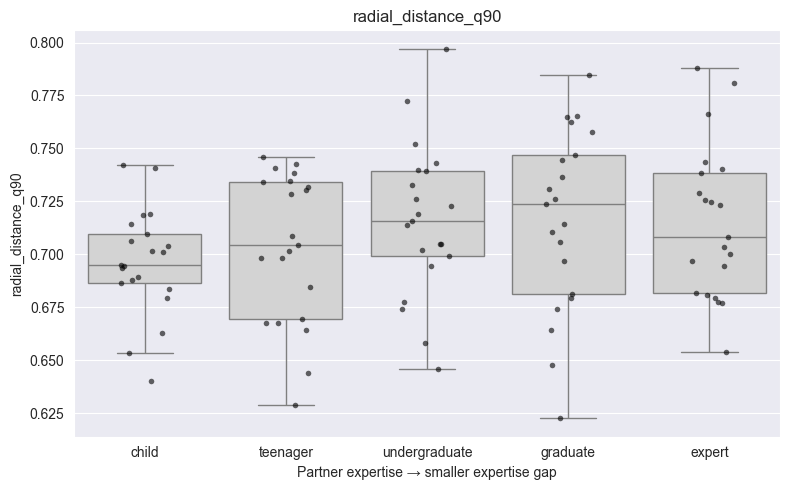
\includegraphics[width=0.85\linewidth]{figures/radial_distance_q90.png}
    \caption{90th-percentile radial distance from the conversation centroid by conversation partner expertise.}
    \label{fig:radial-distance-q90}
\end{figure}

\subsection{Participation Ratio}

  Participation ratio tended to increase as expertise gap decreased as can be seen in figure~\ref{fig:participation-ratio}, indicating higher conversation dimensionality at higher levels of conversation. Participation ratio increased by $\beta= 0.176$ per level increase, with 95\%CI$[0.119, 0.233]$ and a $p_{\mathrm{FDR}} $ of $0.002$. Even with little difference in overall dispersion/variation as seen with the radial distancces, the experts had significantly higher PR values, indicating that even with similar overall dispersions, the variation was structured significantly differently than in expert-novice and other *** conversations. Expert-expert pairs were able to more precisely expand the conversation in controlled ways(they can say more things in more controlled ways). In expert-novice conversations, even though the expert could take the conversation in more directions, their semantic trajectories are limited as they have to scaffold for the novice speaker. This leads to the PR values for expert-novice being significantly lower, even with experts leading the conversations.

\begin{figure}[H]
    \centering
    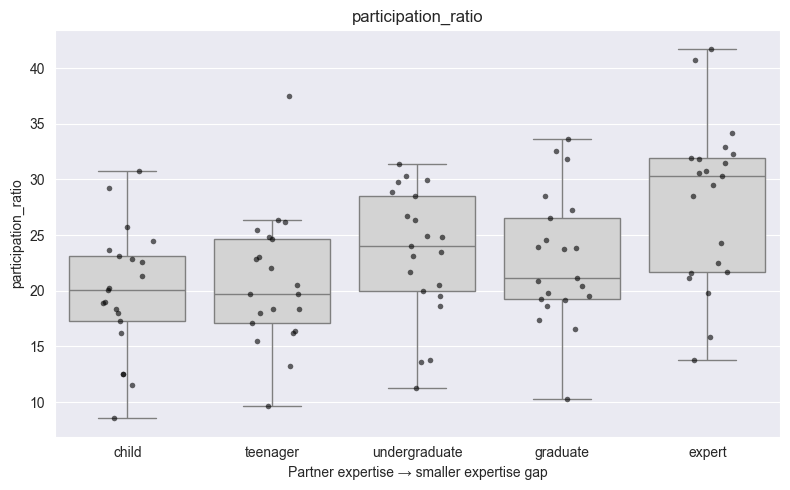
\includegraphics[width=0.85\linewidth]{figures/particioation_ratio_plot.png}
    \caption{Participation ratio of conversation embeddings by conversation partner expertise.}
    \label{fig:participation-ratio}
\end{figure}

\subsection{Statistical Significance}
% Probably rename this later, but it's fine for now

\begin{table}[htbp]
\centering
\small
\caption{Associations between partner expertise and conversational geometry.}
\label{tab:expertise-effects}
\begin{tabular}{llrrrr}
\toprule
Metric & Model & $b_{\mathrm{SD}}$ & 95\% CI
& $p_{\mathrm{boot}}$ & $p_{\mathrm{BH}}$ \\
\midrule
Centroid distance
& Unadjusted     & $-0.364$ & [$-0.465$, $-0.263$] & .001 & .002 \\
& Count-adjusted & $-0.313$ & [$-0.414$, $-0.211$] & .001 & .002 \\
\addlinespace
Median radial distance
& Unadjusted     & $-0.061$ & [$-0.182$, $0.060$]  & .335 & .335 \\
& Count-adjusted & $-0.133$ & [$-0.239$, $-0.027$] & .019 & .025 \\
\addlinespace
Q90 radial distance
& Unadjusted     & $0.141$  & [$0.034$, $0.248$]   & .009 & .014 \\
& Count-adjusted & $0.106$  & [$-0.003$, $0.214$]  & .073 & .083 \\
\addlinespace
Participation ratio
& Unadjusted     & $0.275$  & [$0.179$, $0.370$]   & .001 & .002 \\
& Count-adjusted & $0.176$  & [$0.119$, $0.233$]   & .001 & .002 \\
\bottomrule
\end{tabular}

\medskip
\begin{minipage}{\linewidth}
\footnotesize
\textit{Note.}
For each measure, $b_{\mathrm{SD}}$ represents the change in metric value per one increase in standard deviation.
\end{minipage}
\end{table}

\section{Discussion}

% Summary of main findings

% Interpretation / high level discussion of contraction and ramification.

% Implications. Go through each of the (many!) literatures relevant to this and discuss what this shows. We can drop in a bit of Husserl too :)

% Limitations

% Future directions

\bibliographystyle{plainnat}
\bibliography{horizons}

\end{document}
